%************************************************
%************************************************
%************************************************
% UNOFFICIAL OHIO STATE COLLEGE OF
% ENGINEERING MS/PHD/CANDIDACY TEMPLATE
%************************************************
%************************************************
% Template by Richard Vasques
% Last updated December 2019
%************************************************
%************************************************

% This is a template for my current and future students that will be writing their documents in LaTeX.
% This is an adaptation of the template by Swarnendu Biswas that can be found at https://github.com/swarnendubiswas/ohio-state-coe-dissertation-template.
% This template attempts to follow the rules prescribed by the Graduate School and College of Engineering, and is (hopefully) up to date with the graduate school requirements as of December 2019. 
% This adaptation is intended for students in my research group only, and is not officially supported by The Ohio State University, with no claims being made about its conformity with the current requirements.
% (In fact, this is a hastily put together template, as I do not have the time I
% wish to go deeply into the sty and cls files to make something nicer)

%************************************************
%************************************************

% This file (Dissertation-template) is the source file; that means, the one you need to compile.
% I recommend you name this file after yourself (e.g. Lastname_Dissertation.tex).

%************************************************
%************************************************

% Have the following files in the same folder:
%
% osudissert96-mods.sty
% osudissert96.cls
% This_File.tex (this current file, currently named Dissertation-template.tex, hopefully renamed by you)
% references.bib (this is your bibliography)

%************************************************
%************************************************
% Also, have the subfolders ``texfiles" and ``images".
% In ``images" you will place all figures and images.
% In ``texfiles" you will place all other tex files (duh) of your document,
% including for this template:
% preamble.tex 
% abstract.tex
% acknowl.tex
% vita.tex
% symbols.tex
% introduction.tex
% chapter2.tex
% conclusions.tex
% app1.tex
% and any other tex files you need 

%************************************************
%************************************************

% To change the dissertation to a Master's Thesis, use a documentclass option such as [masters] or [ms].
% To change to a PhD candidacy proposal, use a documentclass option [candidacy].
% The default option is phd.
% Also available are [osudraft] and [twoside].
% As a reminder, documentclass options are a comma-separated list, e.g. \documentclass[ms,osudraft]{osudissert96}

%\documentclass[ms]{osudissert96}
%\documentclass[candidacy]{osudissert96}
\documentclass{osudissert96}

%************************************************
%************************************************

% Put all package definitions in the file Preamble.tex:
\input{texfiles/preamble}
% I have populated the file Preamble.tex with the packages you will
% probably need.
% Feel free to add/change/remove packages according to your needs, as long
% as it works without breaking anything else. 

%************************************************
%************************************************

% It is better to break up the dissertation into multiple files (e.g.,
% one file per chapter, as well as separate files for the abstract,
% acknowledgments, vita, etc.).  These files are brought into the
% document using \include{} statements.  There will be times, however,
% when you don't want to print the ENTIRE dissertation.  You can limit
% what will actually be printed by using the \includeonly{} statement.
% This contains a list of the files you want printed.  Any file NOT
% listed will not be printed.  However, all page numbers, references,
% etc., will be preserved as though all the files were actually
% printed. For example, the line below would result only in chapters 
% "introduction" and "chapter2" being printed (if it were uncommented).

% \includeonly{introduction,chapter2}

%************************************************
%************************************************

% UPDATED TEXT (2010):
% In the newest format, titles should be title case everywhere.
\renewcommand\typesetChapterTitle[1]{#1}

%************************************************
%************************************************

\begin{document}

% First, declare the parts of your title page

%Your full name
\author{Firstname Midname Lastname}

%Title of your work
\title{Ohio State College of Engineering MS/PhD/Candidacy Dissertation Template}

% Your Degrees thus far, not including the one for this document. Ex: B.S., B.Sc., B.E., M.Sc., M.S., etc.
\authordegrees{B.S., M.S.}  

%Program name (TeX will add the words "Graduate Program in"
\unit{Nuclear Engineering}

% Committee members
\advisorname{Richard Vasques} %This should probably be me
\member{Someone 1, Co-Advisor} % Only use Co-Advisor if needed; otherwise just enter the name of the committee member. 
\member{Someone 2}
\member{Maybe Someone 3}

% The following creates the title page
\maketitle

%************************************************
%************************************************

% Next, EITHER a copyright or BLANK page.
%
%   The following creates a page used to copyright your dissertation
%
%   BACKGROUND: Even without this copyright page, your dissertation will
%               carry a common-law copyright. However, if your
%               dissertation ends up seeing wide distribution, your
%               common-law copyright is at risk of being expunged.
%               Adding this copyright page prevents that from happening.
%
%               There are NO DOWNSIDES to including a copyright page as
%               your document is automatically copyright by law anyway.
%               However, this copyright page is OPTIONAL. If you get rid
%               of it, uncomment the \blankpage that follows it so that
%               there is a blank page here. The graduate school requires
%               a page here that is either blank or carries the
%               copyright.
%
%   IMPORTANT NOTE: The graduate school requires either a copyright page
%                   here or a BLANK PAGE here. If you get rid of the
%                   copyright, uncomment the \blankpage that follows it.
%                   You should NOT have BOTH uncommented.
%

% If you get rid of \disscopyright, restore the \blankpage line after it
\disscopyright{}
%\blankpage

%************************************************
%************************************************

% Bring in abstract from separate file named ``abstract.tex''
 \begin{abstract}
	 %Abstract.

This is your abstract.
Fill it accordingly. 

\lipsum[1-3]


 \end{abstract}

%************************************************
%************************************************

%  Dedication goes after the abstract. Dedication is not needed (up to you), and
%should not be present in candidacy proposal. Refrain from adding a dedication
%page until after the defense.
\dedication{\emph{Dedicated to the Avengers for killing Thanos.}}

%************************************************
%************************************************

% UPDATED TEXT (2010):
%  The graduate school does not require an external abstract. If this
%  changes, follow the old instructions below.
%
% HISTORICAL TEXT (1996):
%  Uncomment the three lines below to generate the external abstract.  Two
%  copies of this must be turned in to the graduate school.  These lines can
%  be placed pretty much anywhere, since the page numbering should be
%  independent of the rest of the thesis
%

% \begin{externalabstract}
%   %Abstract.

This is your abstract.
Fill it accordingly. 

\lipsum[1-3]


% \end{externalabstract}

%************************************************
%************************************************

% If this is a PhD or MS document, include the following:
% Bring in Acknowledgment from separate file named ``acknowl.tex'' or some other name you defined
\begin{acknowledgements}
I thank my friends and family, without whom this work would have been completed two years earlier.

In reality, this is the only page of the dissertation of which the author has full control.
You can write anything you want here, and no one can tell you it is wrong (except if the margins don't line up!!!!).
\end{acknowledgements}

 % Do not include for a candidacy proposal, and 
%refrain from including it until after the defense.

%************************************************
%************************************************

% Bring in Vita from separate file named ``vita.tex'' or some other name you defined
\begin{vita}

\dateitem{August 2016}{B.S. in something, The Ohio State University}

\dateitem{Some date}{Some degree, Some place}

\dateitem{September 2016 to present}{Graduate Research Associate,\\The Ohio State University}

\begin{publist}

%% UPDATE FOR 2010:
%  Grad school only wants research publications, and it only wants those
%  research pubs that are actually published. Accepted or ``to appear''
%  publications don't count. If they look closely, they'll tell you to
%  remove any publications that aren't in print. Having said that, they
%  probably won't look that closely unless you put a really long list
%  here. You're tempting fate if you add instructional publications
%  though.

\researchpubs{}

\pubitem{F.M.~Lastname, J.~Doe, and R.~Vasques, ``Some Cool Title for a Paper," Journal Name, vol.~99, pp.~11-22, 2018.
}

% \instructpubs
%
% \pubitem{B.~Simpson, ed.,
% \newblock ``Lab notes for Cow Science 101'', 1909.}

\end{publist}

\begin{fieldsstudy}

% The \majorfield* uses the unit specified in the \unit command used
% earlier in your document.
 \majorfield*

%If you want to use different units, use the
% second form shown below:
%\majorfield{Computer Science and Engineering}
%\begin{studieslist}
%\studyitem{XX}{Prof.\ XX}
%\studyitem{YY}{Prof.\ YY}
%\studyitem{ZZ}{Prof.\ ZZ}
%\end{studieslist}

%% Note:  If there were only one extra field of study, the list
  %% would best be done using the following command:
%%
%%  \onestudy{Only Topic}{Only Professor}
%%

\end{fieldsstudy}

\end{vita}
 % Do not include for a candidacy proposal

%************************************************
%************************************************

% Make the Table of Contents and lists
\tableofcontents %Table of contents
\listoftables %List of tables (automatic)
\listoffigures %List of figures (automatic)
\begin{listofsymbols}
	 $\psi$ \dotfill Angular Flux

$\phi$ \dotfill Scalar Flux %List of symbols (entered manually in
	 % symbols.tex)
 \end{listofsymbols}

%************************************************
%************************************************

 % The following is a list of chapters.  Each is brought in from a
 % separate file using the \include{} command.

\newpage
\chapter{Introduction}\label{chap_intro}

This is your introduction chapter.
You are allowed to make sections and subsections.

\section{Something Basic}\label{sec_basic}
This is a section.

\subsection{Something even more basic}\label{subsec_basic}

This is a subsection.

\section{Another Section}\label{sec_another}

This is another section.

     %Introduction Chapter

\newpage
\chapter{Neutron Spectrum Unfolding}\label{chap_chap2}
This Chapter will contain all of the current neutron spectrum unfolding techniques, including the strengths and weaknesses of each.

\section{Radiation Interaction with Matter}\label{radiation_basics}
Radiation interacts with stuff

\section{Spectrum Unfolding}\label{spectrum_unfolding}
Spectrum unfolding requires math.

\subsection{Detector Response Matrix}\label{subsec_drm}

\section{MAXED}\label{MAXED_description}
An introduction about MAXED and the reasons it was developed will go here.

\subsection{Description of the math of detector response unfolding}\label{MAXED_math}
Talk about dual annealing, the maximum entropy method, $\chi^2$ method.

\subsection{Passive Neutron Spectrometer Response}\label{PNS_response}
The Passive Neutron Spectrometer provides similar capabilities to multisphere neutron spectrometers (like Bonner spheres), albeit in a single sphere of material. With the 55 TLDs arranged along the three Cartesian axes, each detector has a different thickness of material separating it from a potential neutron source. This arrangement effects a different response in each of the TLDs, which can be utilized in unfolding techniques.

A typical depth-averaged (I'll have described this in an earlier chapter/section) detector response from the PNS is shown in Figure \ref{example_PNS_dr}.

\begin{figure}[H]
  \centering
  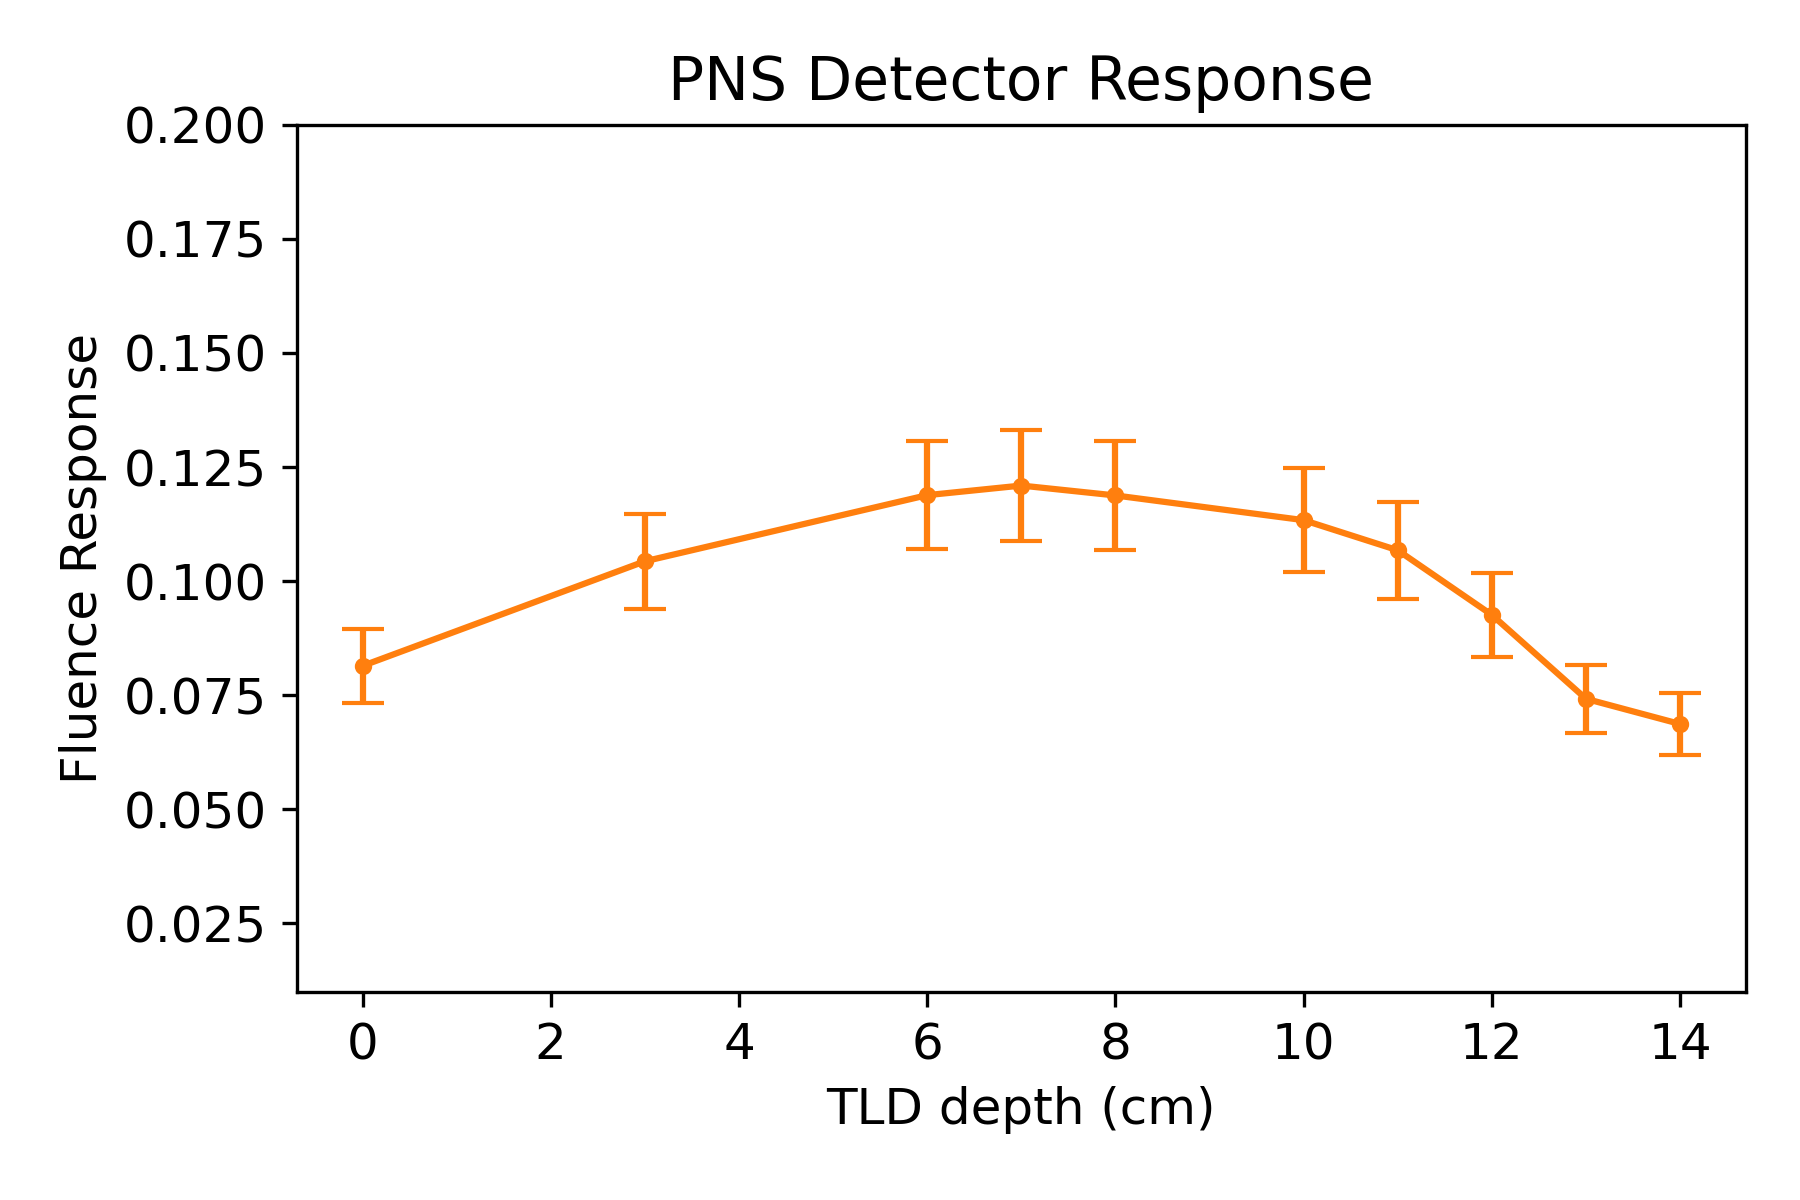
\includegraphics[scale=0.9]{images/Example_PNS_dr.png}
  \caption{A depth-averaged detector response from the PNS in the presence of a Cf-252 neutron source.} \label{example_PNS_dr}
\end{figure}

\subsection{Unfolding the Detector Response}
(The math will be described in Section \ref{MAXED_math})
The detector response from Figure \ref{example_PNS_dr} was used to unfold the neutron spectrum. As mentioned earlier, this detector response was achieved in the presence of a Cf-252 source. Knowing the correct spectrum allows for a good measurement of the accuracy of the algorithm.
The inputs needed for MAXED to unfold the spectrum is a detector response, an initial guess at what the spectrum should be, and, as mentioned in Section \ref{subsec_drm}, a detector response matrix. The following sections will show the accuracy of MAXED when the guess spectrum is varied and showcases the extreme sensitivity to the initial guess.

Because the true spectrum is known, the accuracy of the output of MAXED can be calculated and compared using the modal assurance criterion (MAC). (Put more information about it here) It gives a range (0 1], 1 being an exact match between two sets of data and anything lower is less similar.

\begin{align}\label{eq:MAC}
MAC = \frac{|(Spectrum_{unfolded})^T(Spectrum_{true})|^2}{((Spectrum_{unfolded})^T(Spectrum_{unfolded}))((Spectrum_{true})^T(Spectrum_{true}))} \,.
\end{align}

\subsection*{Using the true spectrum}
An initial point to check for the accuracy of MAXED is by using the true spectrum as the initial guess. The values for this spectrum were taken from the IAEA document Compendium of Neutron Spectra and Detector Responses for Radiation Protection Purposes \cite{iaea_spec}. Barring any other interactions, the MAXED code should get 100\% accuracy on this example, but because the environment surrounding the PNS will reflect neutrons and affect the detector response, there will still be error. The results of this unfolding is shown in \ref{MAXED_result_PlaneDRM_gs100Cf}.
\begin{itemize}
\item DRM: Plane source DRM
\item Guess Spectrum: Cf-252 spectrum
\end{itemize}

\begin{figure}[htb]
  \centering
  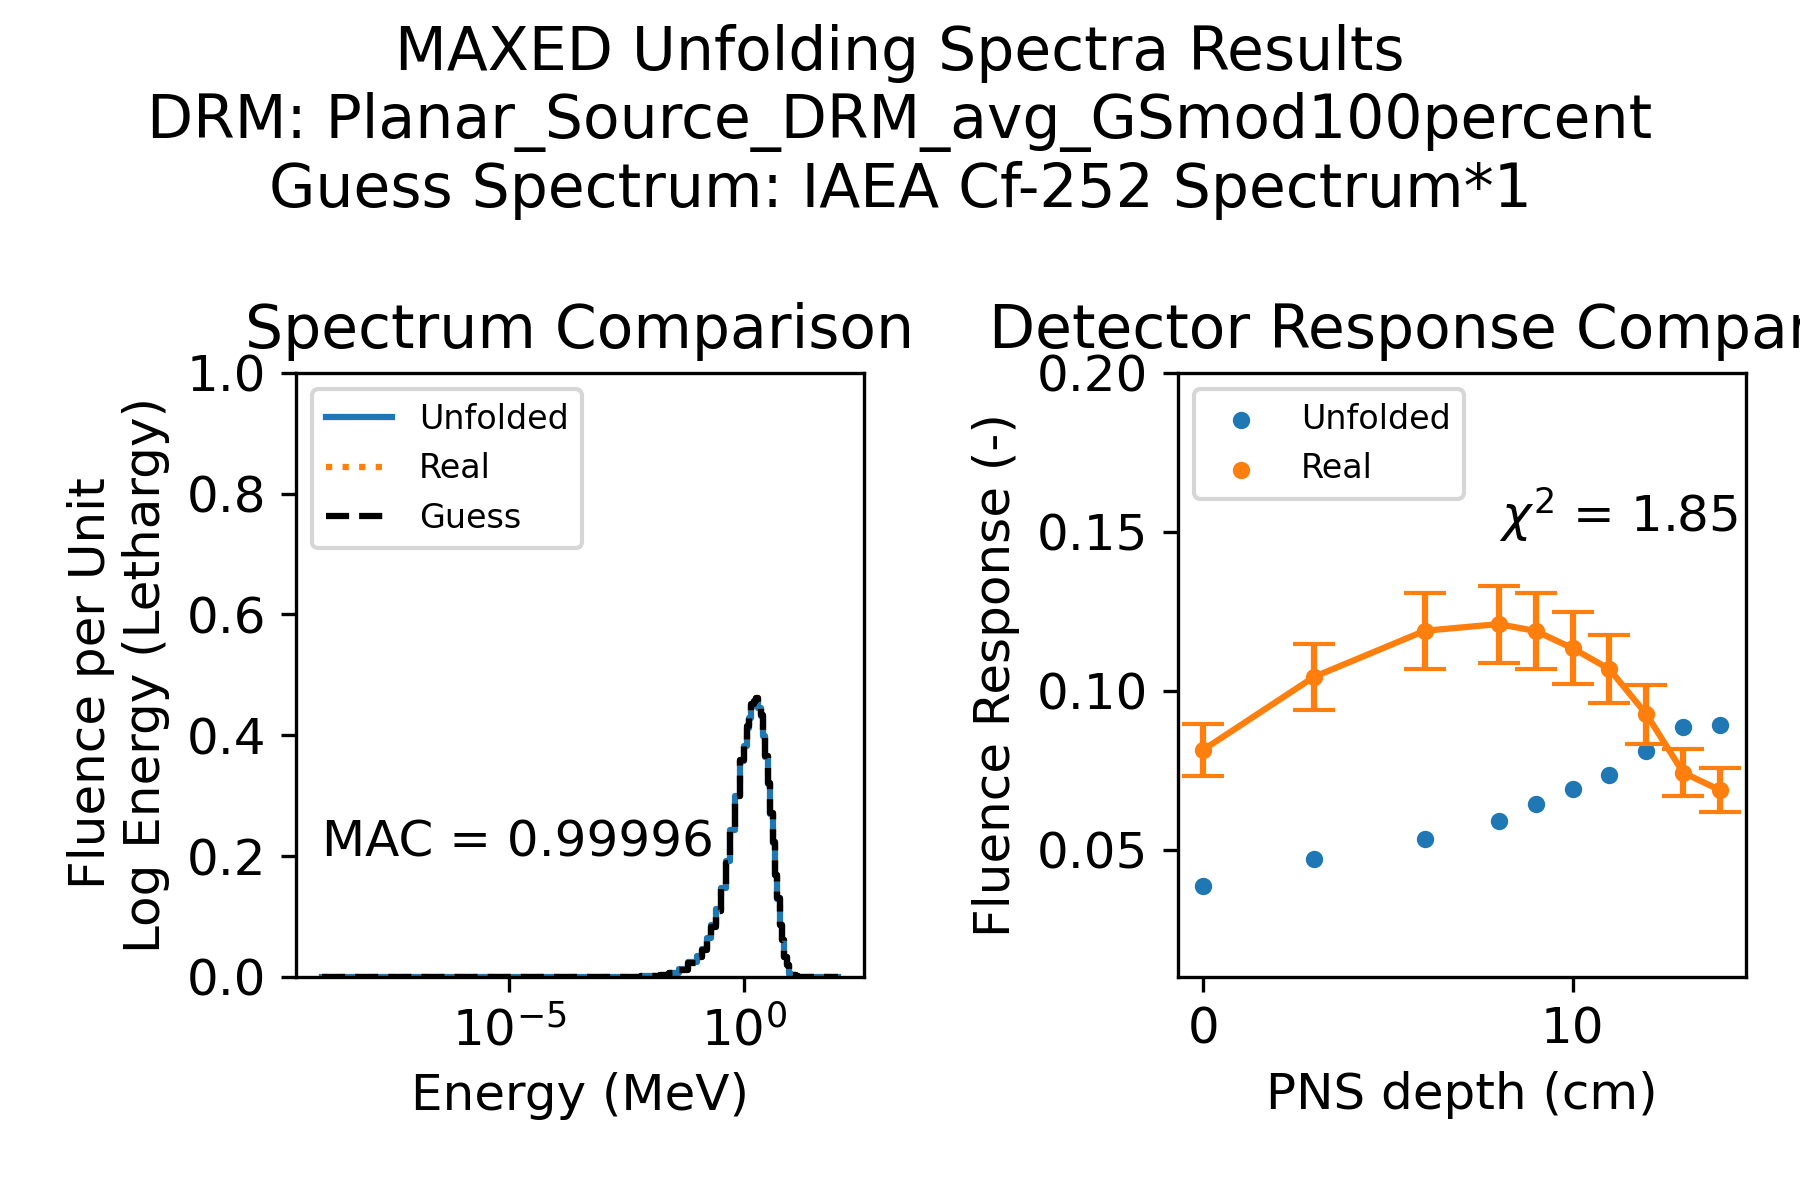
\includegraphics[scale=0.8]{images/Planar_Source_DRM_avg_GSmod100percent_IAEA Cf-252 Spectrum_0.png}
  \caption{The results of the MAXED algorithm using a Cf-252 guess spectrum.} \label{MAXED_result_PlaneDRM_gs100Cf}
\end{figure}

\subsection*{Using the true spectrum with a different DRM}
Following the above example but with a DRM developing using a spherical source surrounding the PNS and directing neutrons inward. Both are very accurate, with MAC numbers very close to 1. Results are in Figure \ref{MAXED_result_sphereDRM_gs100Cf}
\begin{itemize}
\item DRM: Sphere source DRM
\item Guess Spectrum: Cf-252 spectrum
\end{itemize}

\begin{figure}[htb]
  \centering
  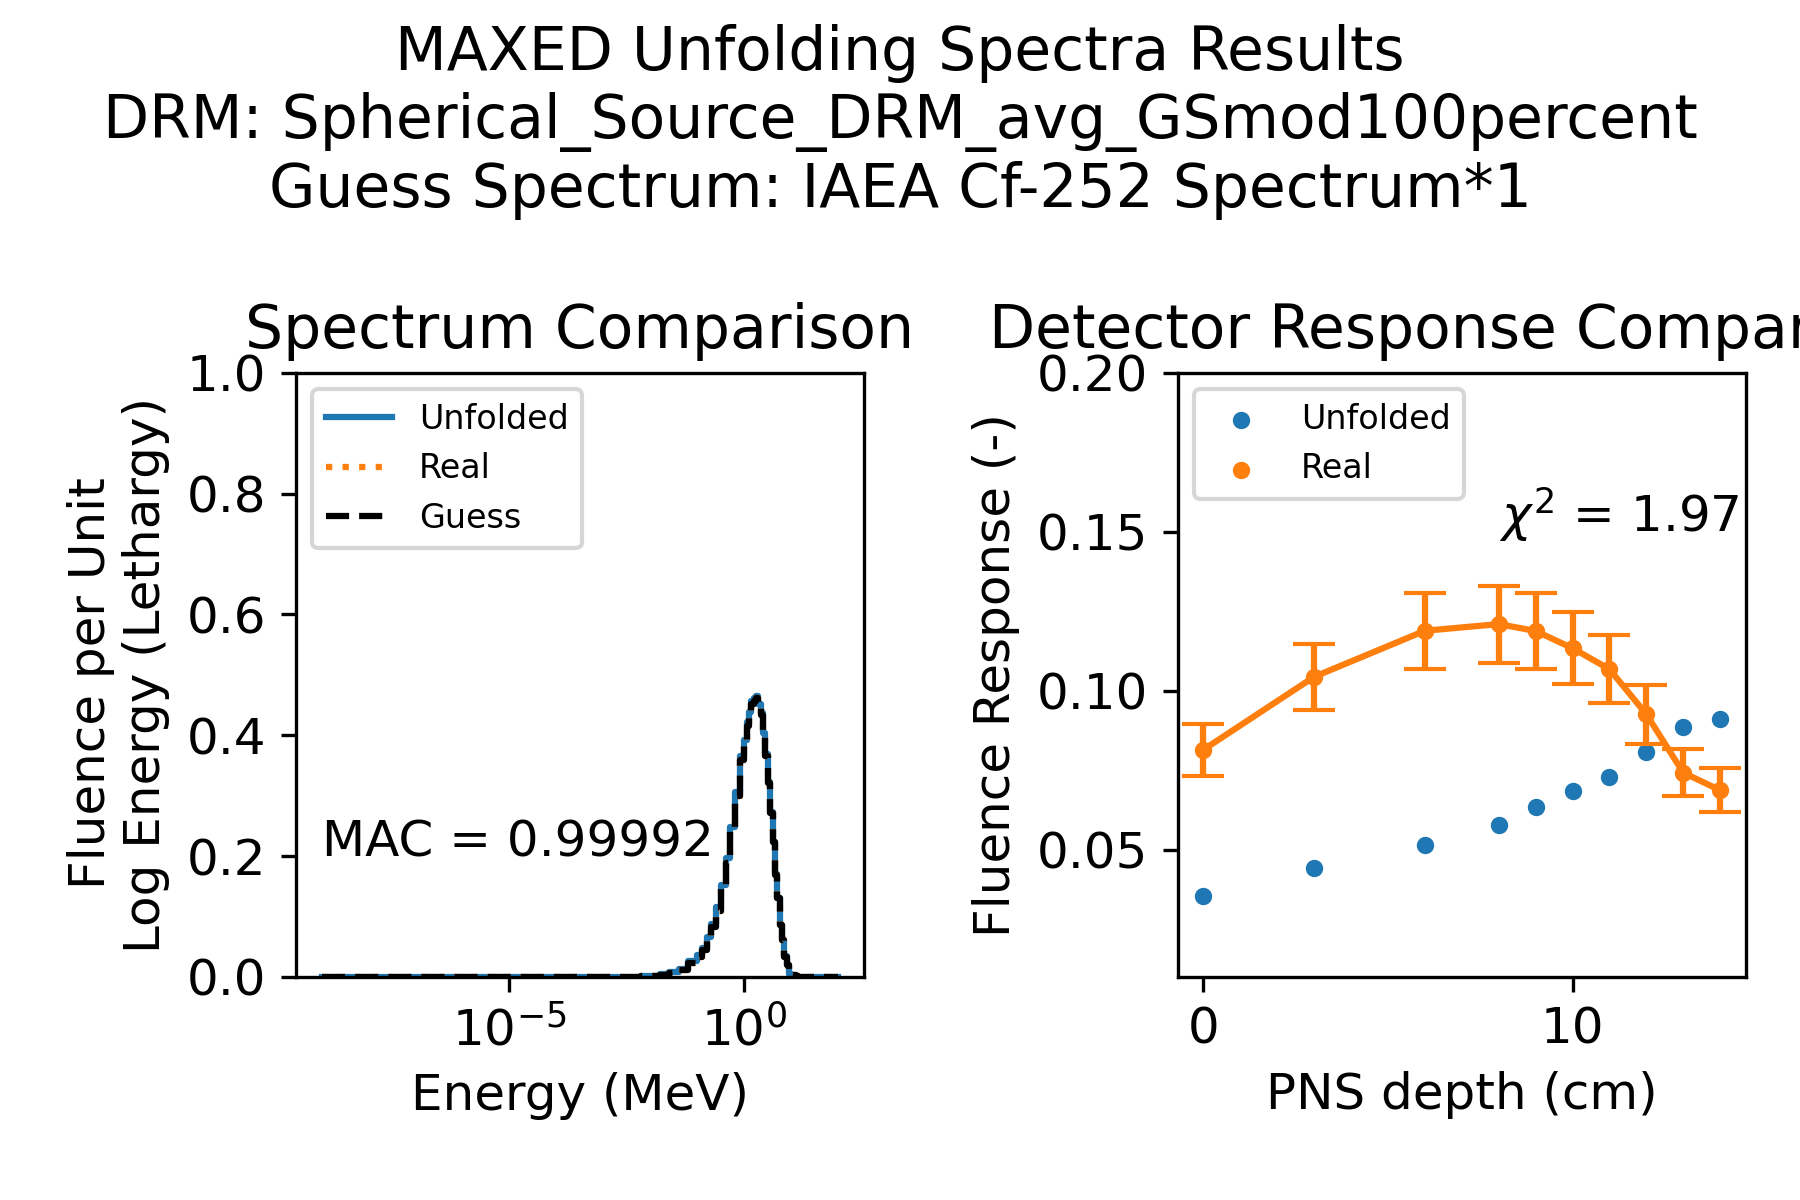
\includegraphics[scale=0.8]{images/Spherical_Source_DRM_avg_GSmod100percent_IAEA Cf-252 Spectrum_0.png}
  \caption{The results of the MAXED algorithm using a Cf-252 guess spectrum.} \label{MAXED_result_sphereDRM_gs100Cf}
\end{figure}

\subsection*{Using the true spectrum multiplied by 0.9}
Running MAXED with the plane-source DRM and using a modified Cf-252 spectrum as the input guess spectrum. The modification was performed by multiplying the spectrum by 0.9. Results are in Figure \ref{MAXED_result_planeDRM_gs90Cf}
\begin{itemize}
\item DRM: Plane source DRM
\item Guess Spectrum: Cf-252 spectrum * 0.9
\end{itemize}

\begin{figure}[htb]
  \centering
  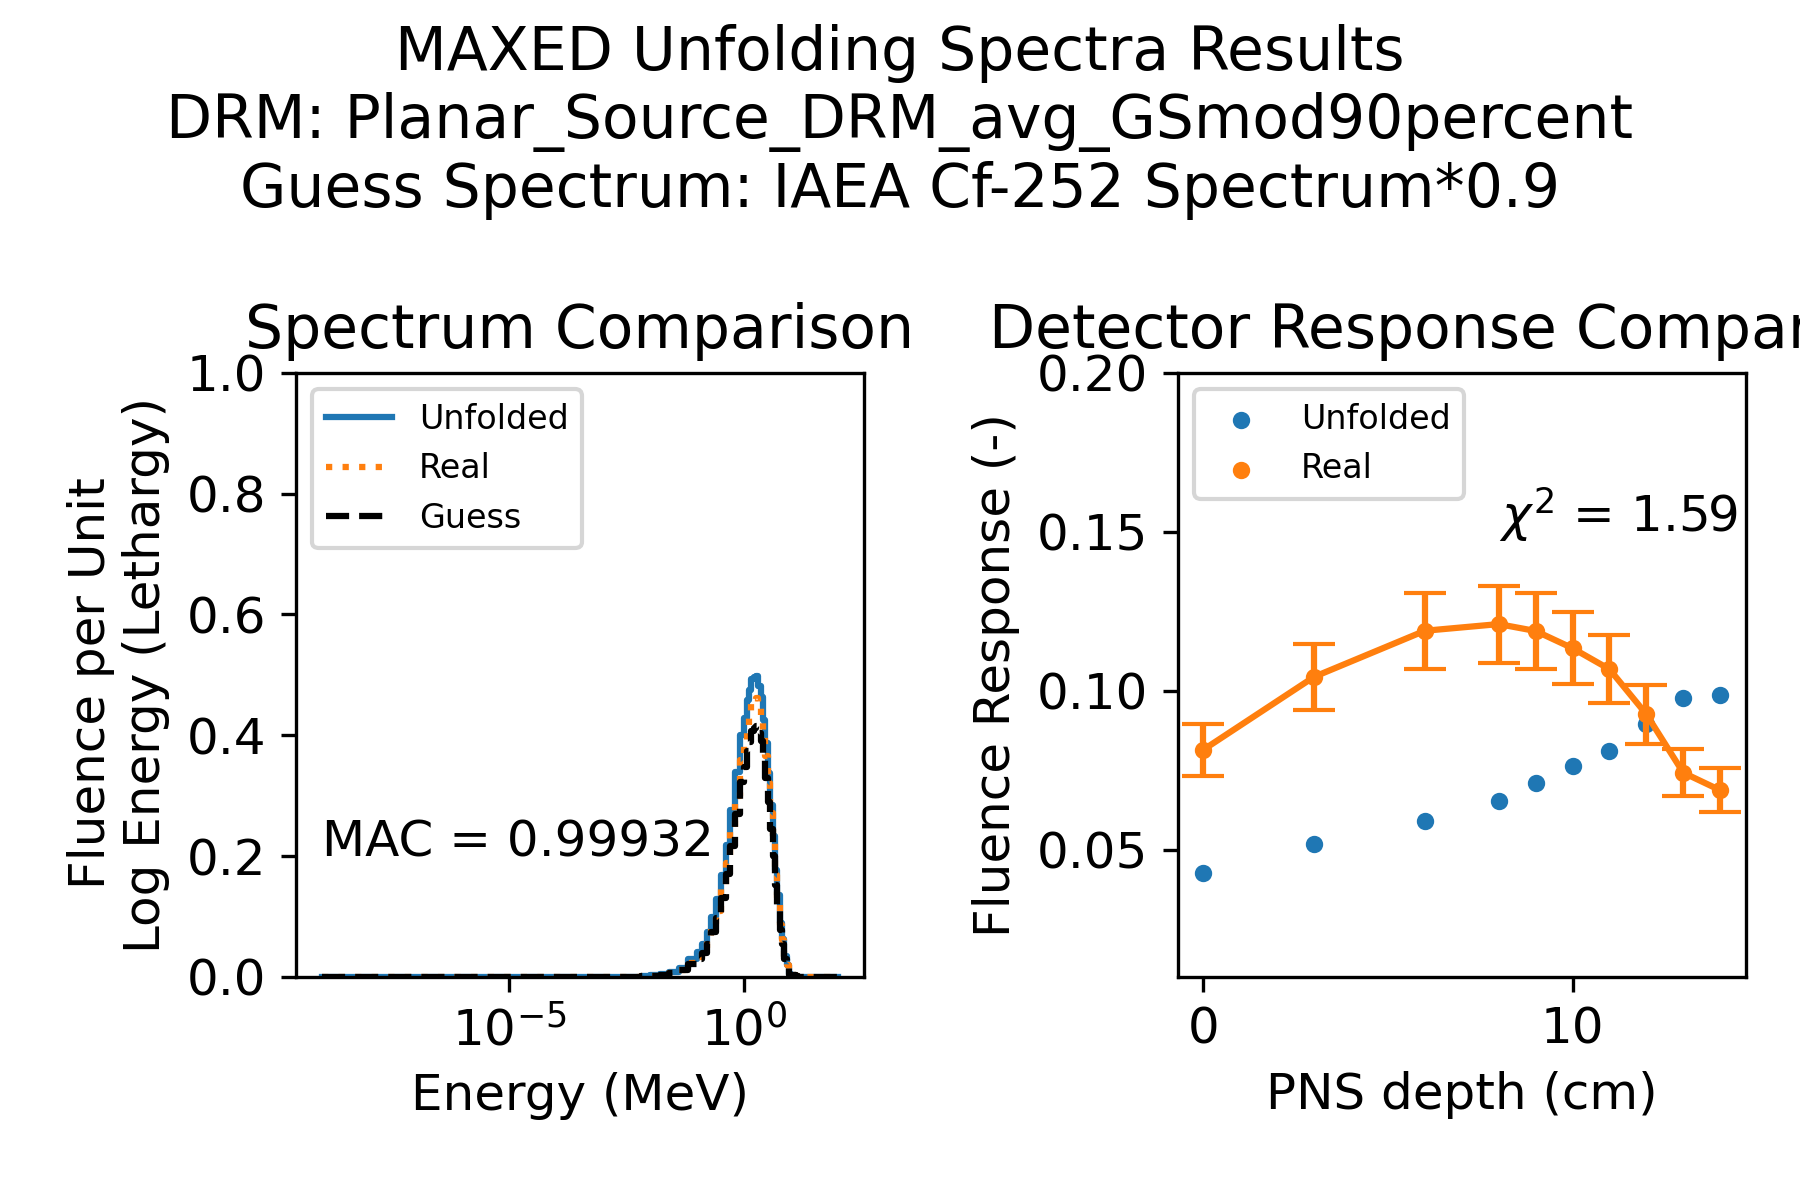
\includegraphics[scale=0.8]{images/Planar_Source_DRM_avg_GSmod90percent_IAEA Cf-252 Spectrum_0.png}
  \caption{The results of the MAXED algorithm using a modified Cf-252 guess spectrum.} \label{MAXED_result_planeDRM_gs90Cf}
\end{figure}

\subsection*{Using the true spectrum multiplied by 0.5}
Running MAXED with the plane-source DRM and using a modified Cf-252 spectrum as the input guess spectrum. The modification was performed by multiplying the spectrum by 0.5. Results are in Figure \ref{MAXED_result_planeDRM_gs50Cf}
\begin{itemize}
\item DRM: Plane source DRM
\item Guess Spectrum: Cf-252 spectrum * 0.5
\end{itemize}

\begin{figure}[htb]
  \centering
  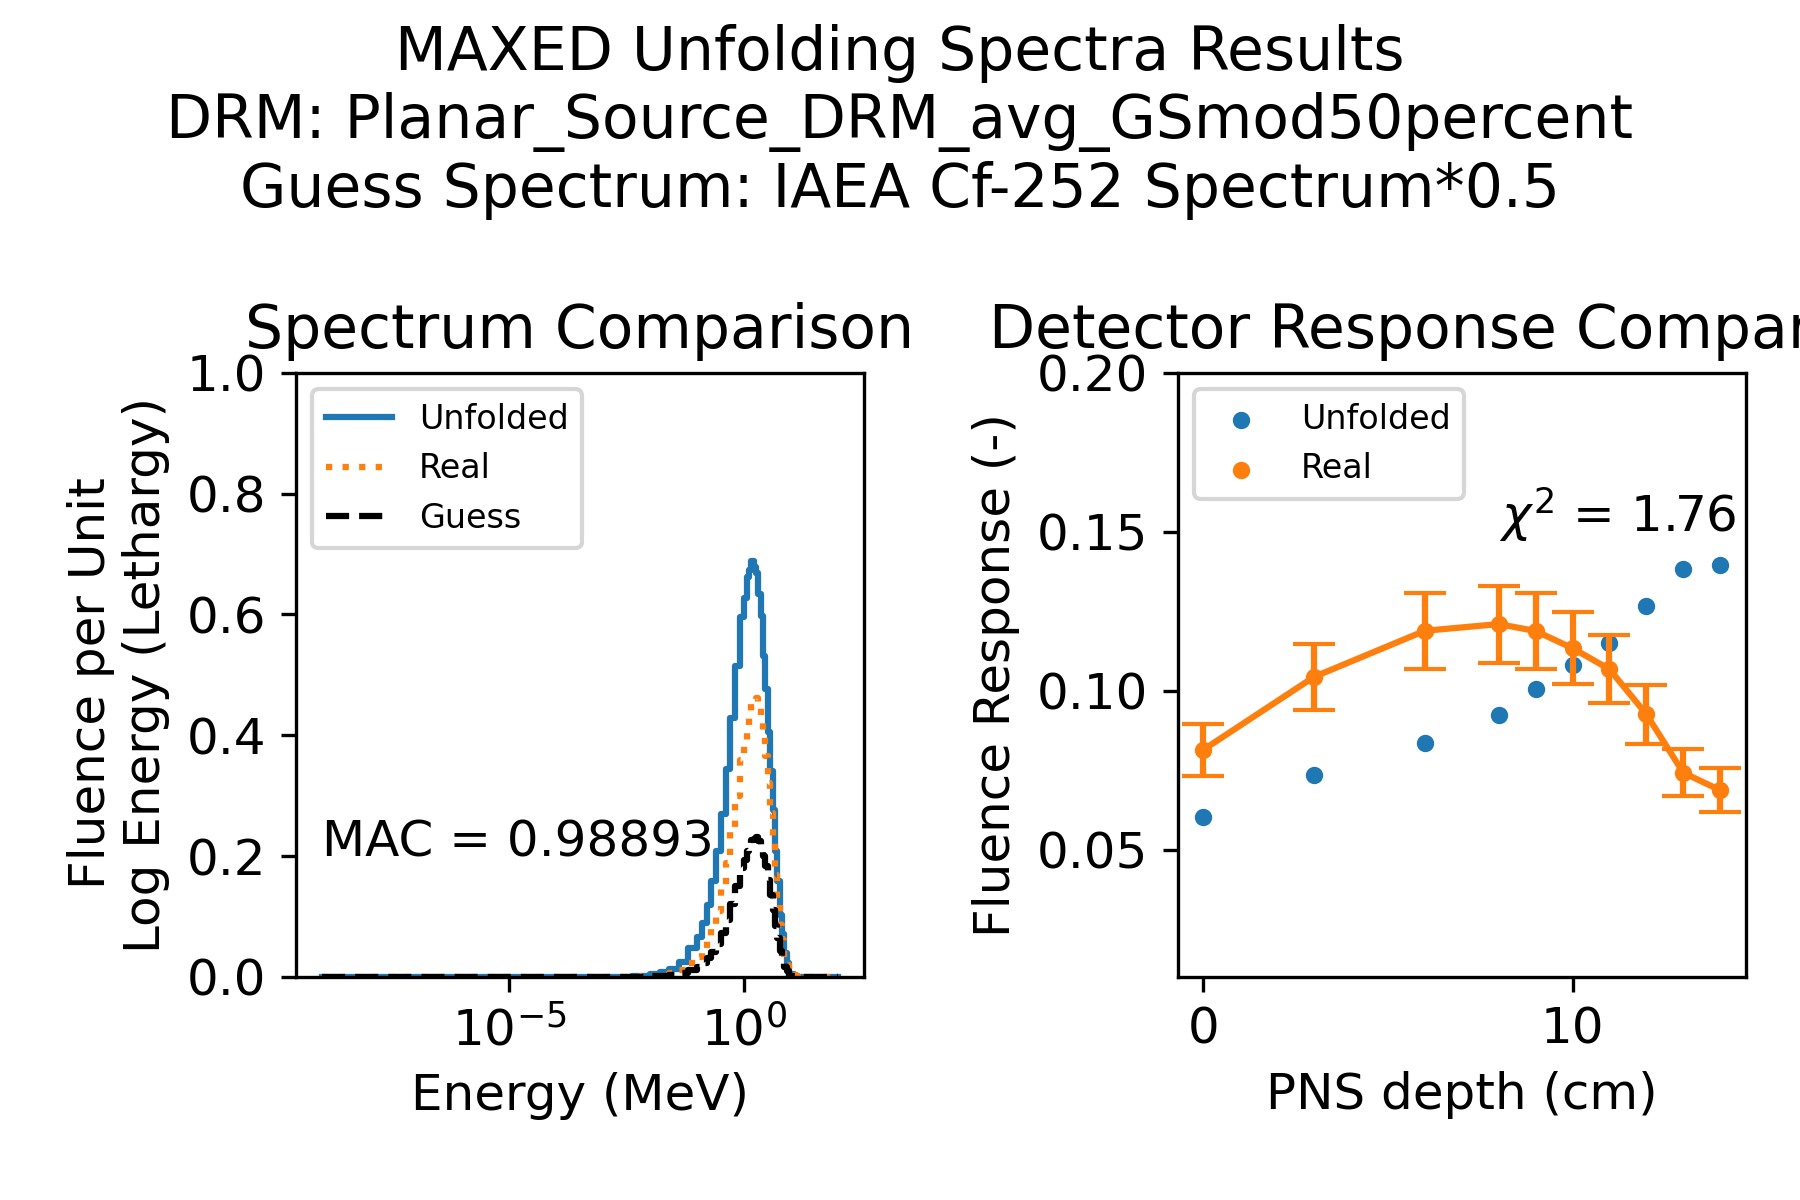
\includegraphics[scale=0.8]{images/Planar_Source_DRM_avg_GSmod50percent_IAEA Cf-252 Spectrum_0.png}
  \caption{The results of the MAXED algorithm using a modified Cf-252 guess spectrum.} \label{MAXED_result_planeDRM_gs50Cf}
\end{figure}

\subsection*{Using a D2O moderated Cf-252 spectrum}
Running MAXED with the plane-source DRM and using a D2O moderated Cf-252 spectrum. Notice that the MAC number is much smaller than 1. Results are in Figure \ref{MAXED_result_planeDRM_gs100D2OmodCf}
\begin{itemize}
\item DRM: Plane source DRM
\item Guess Spectrum: D20 moderated Cf-252 spectrum
\end{itemize}

\begin{figure}[htb]
  \centering
  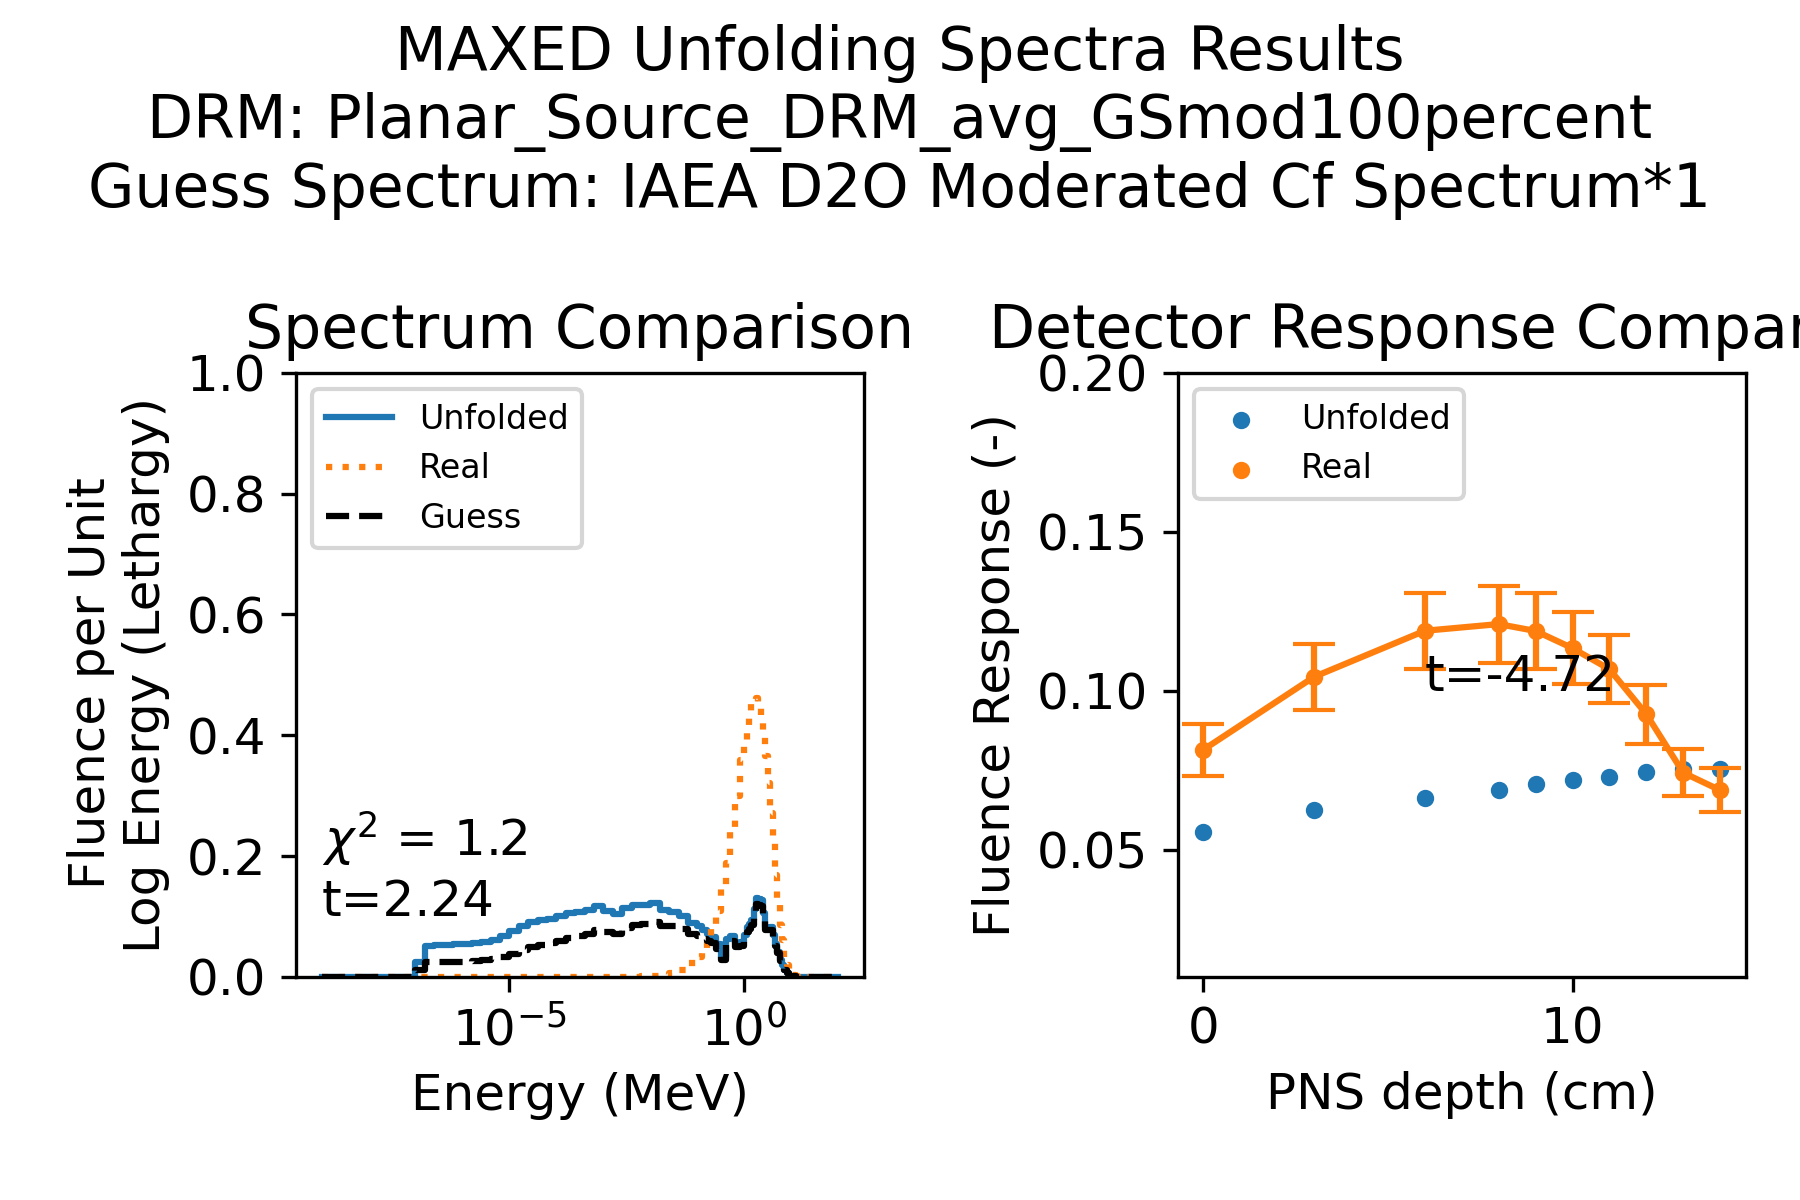
\includegraphics[scale=0.8]{images/Planar_Source_DRM_avg_GSmod100percent_IAEA D2O Moderated Cf Spectrum_0.png}
  \caption{The results of the MAXED algorithm using a D20 moderated Cf-252 guess spectrum.} \label{MAXED_result_planeDRM_gs100D2OmodCf}
\end{figure}

\subsection*{Using a H2O moderated PuBe spectrum}
Running MAXED with the plane-source DRM and using a H2O moderated PuBe spectrum. Notice that the MAC number is much smaller than 1. Results are in Figure \ref{MAXED_result_planeDRM_gs100H2OmodPuBe}
\begin{itemize}
\item DRM: Plane source DRM
\item Guess Spectrum: H2O moderated PuBe spectrum
\end{itemize}

\begin{figure}[htb]
  \centering
  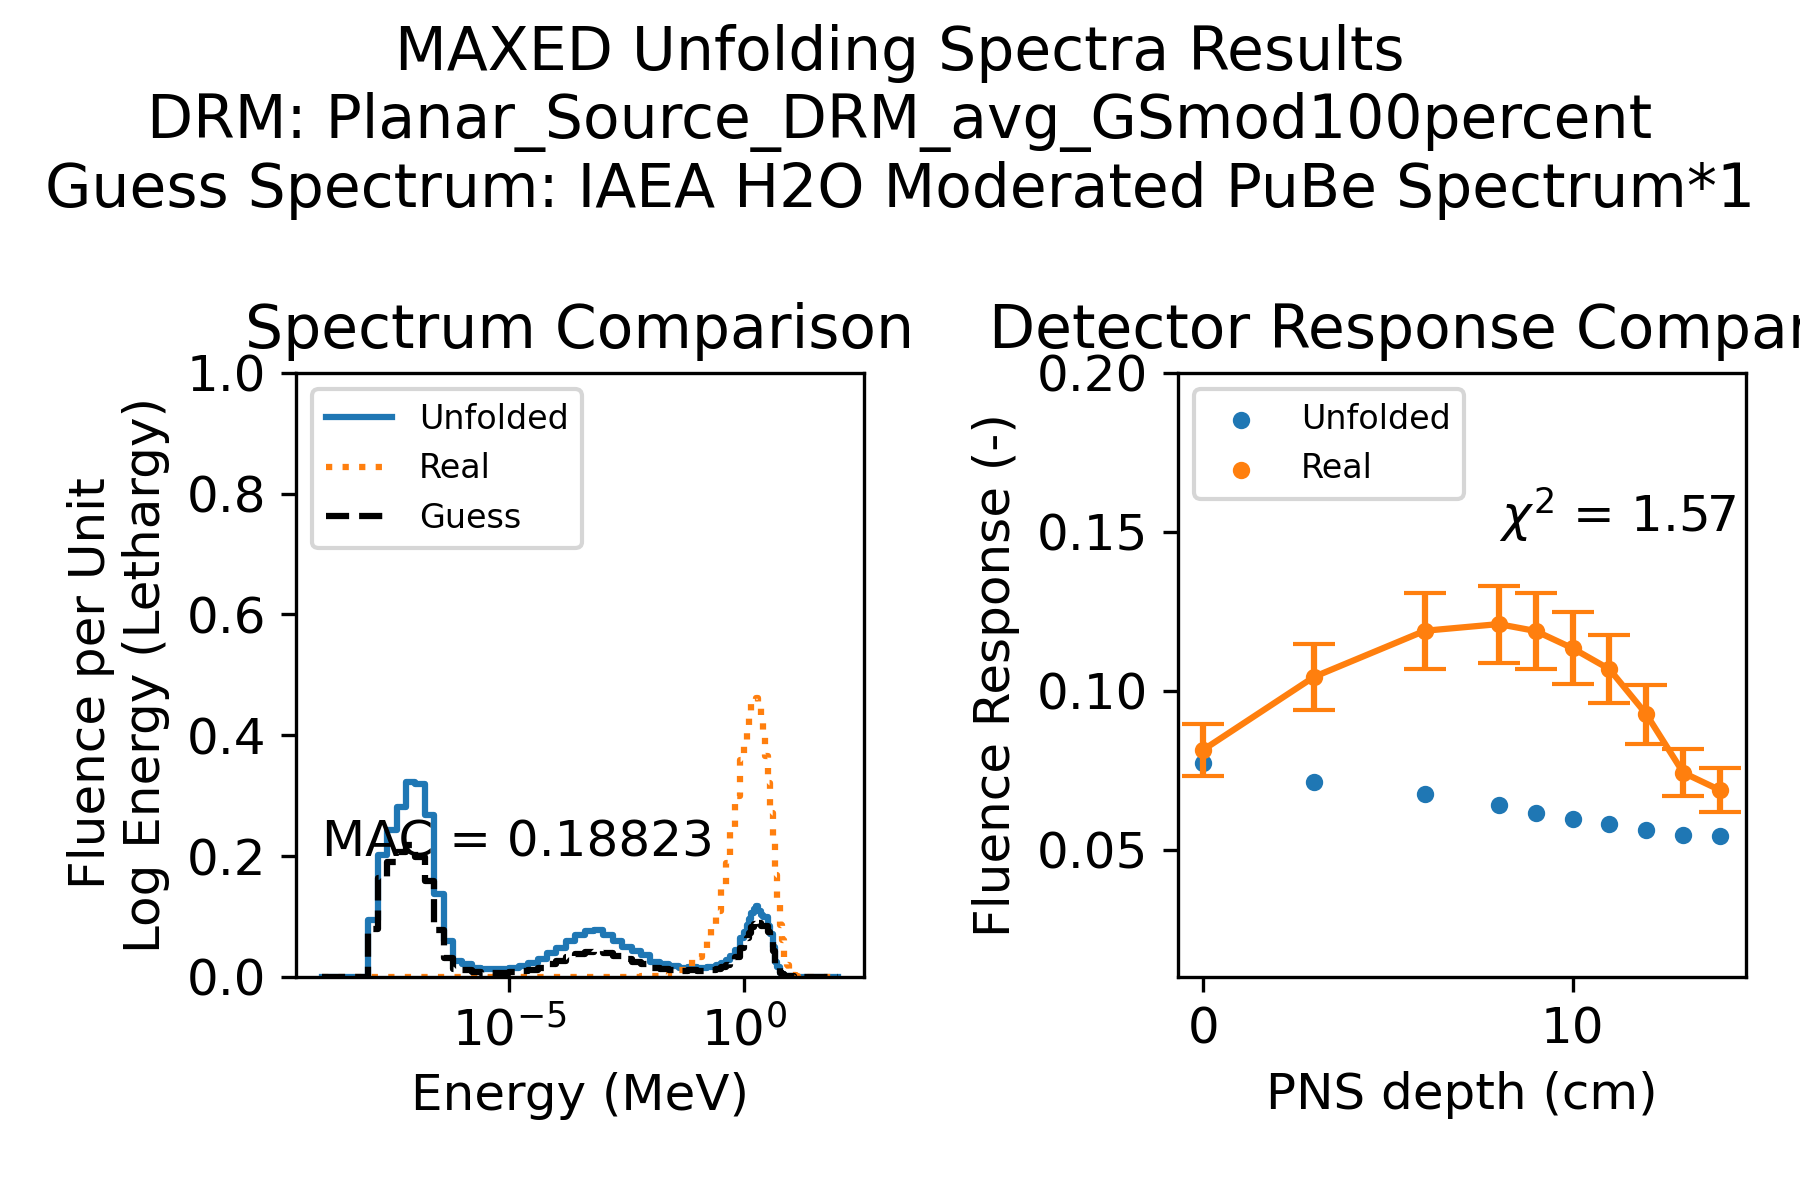
\includegraphics[scale=0.8]{images/Planar_Source_DRM_avg_GSmod100percent_IAEA H2O Moderated PuBe Spectrum_0.png}
  \caption{The results of the MAXED algorithm using a H2O moderated PuBe guess spectrum.} \label{MAXED_result_planeDRM_gs100H2OmodPuBe}
\end{figure}

\subsection*{Using a randomly generated DRM}
Once a different spectrum is used for input, the output of MAXED becomes highly inaccurate. Another test of the robustness is to try using a randomly generated DRM. The results are in Figure \ref{MAXED_result_randomDRM_gs100Cf}. 
\begin{itemize}
\item DRM: Random DRM
\item Guess Spectrum: Cf-252
\end{itemize}

\begin{figure}[htb]
  \centering
  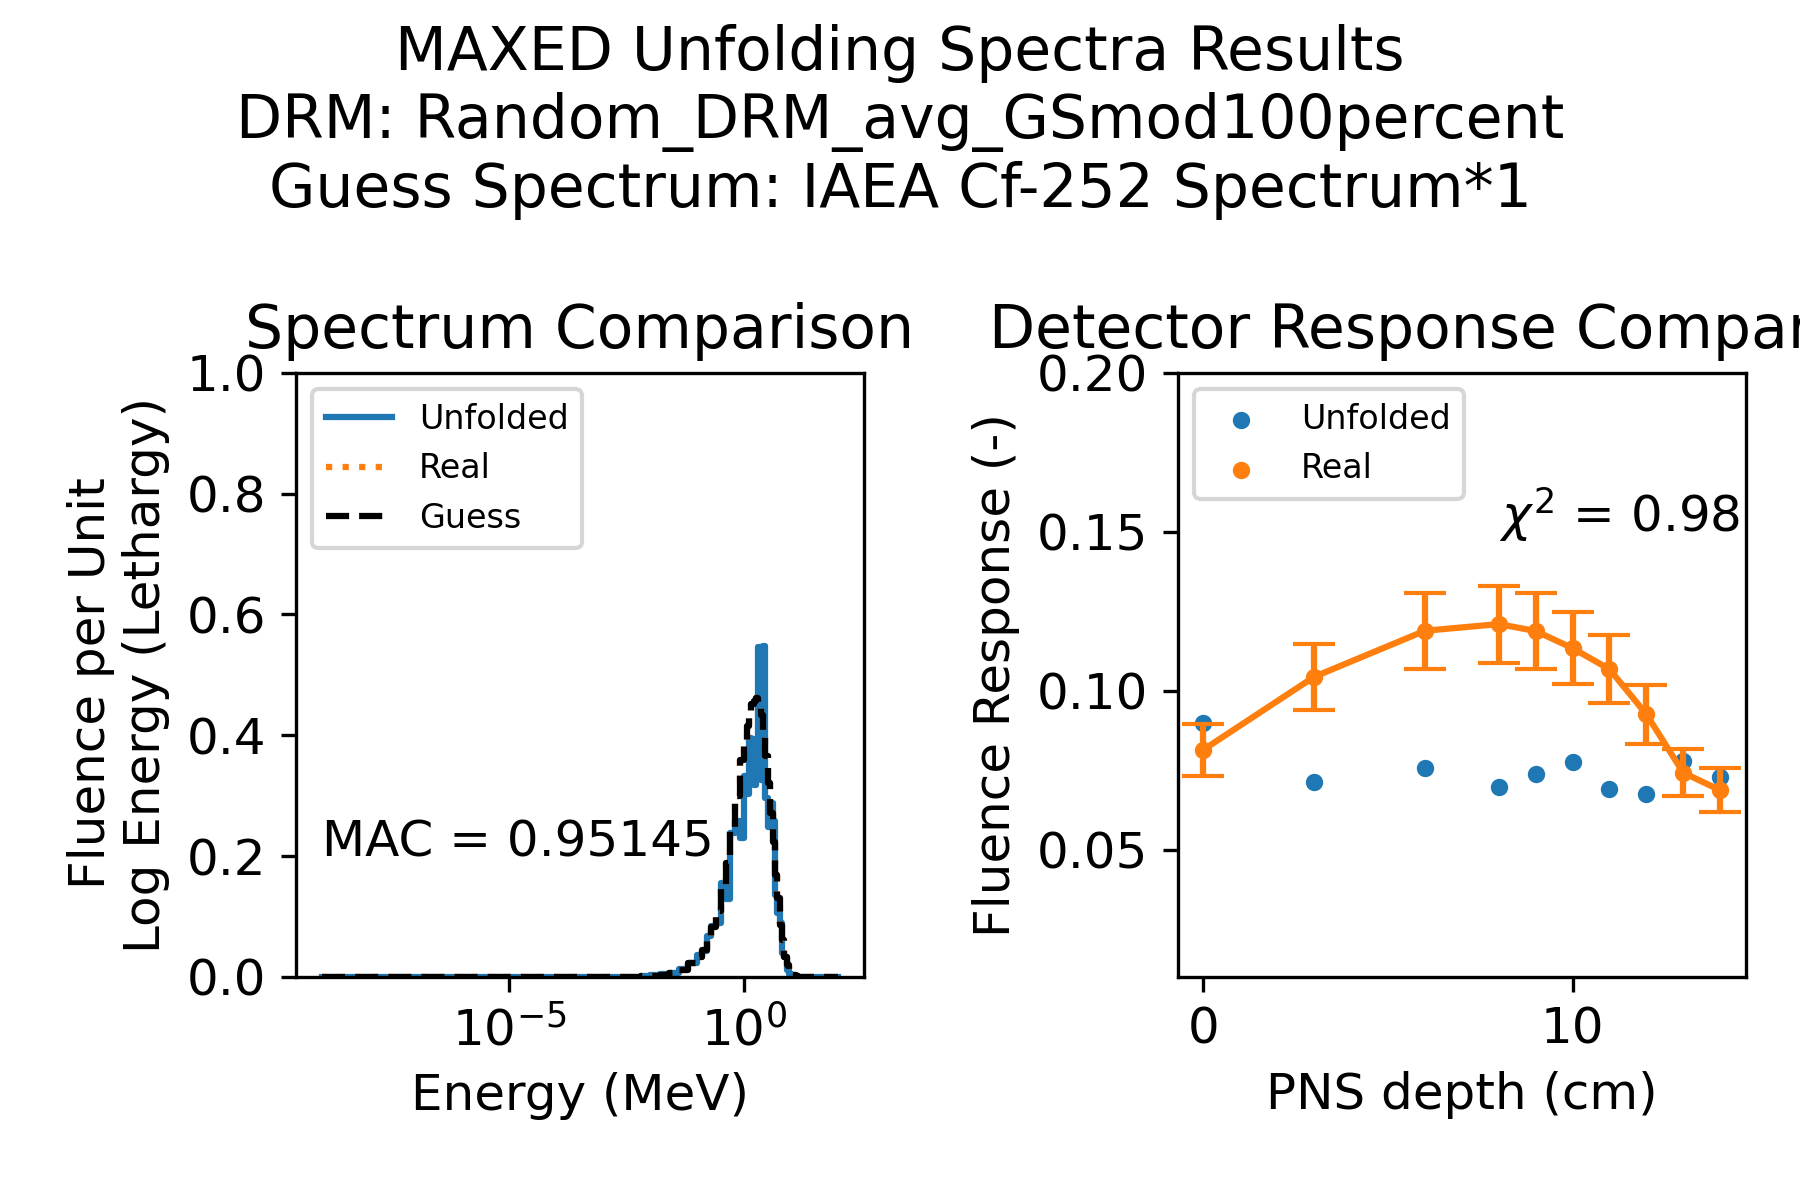
\includegraphics[scale=0.8]{images/Random_DRM_avg_GSmod100percent_IAEA Cf-252 Spectrum_0.png}
  \caption{The results of the MAXED algorithm using a Cf-252 guess spectrum and a randomly generated DRM.} \label{MAXED_result_randomDRM_gs100Cf}
\end{figure}

\subsection*{Using a randomly generated DRM and modified guess spectrum}
The effects of the random DRM are even more visible when the true spectrum is modified like above. In this case, the Cf-252 spectrum is multiplied by 0.5 and the results are in Figure \ref{MAXED_result_randomDRM_gs50Cf}. 
\begin{itemize}
\item DRM: Random DRM
\item Guess Spectrum: Cf-252 * 0.5
\end{itemize}

\begin{figure}[htb]
  \centering
  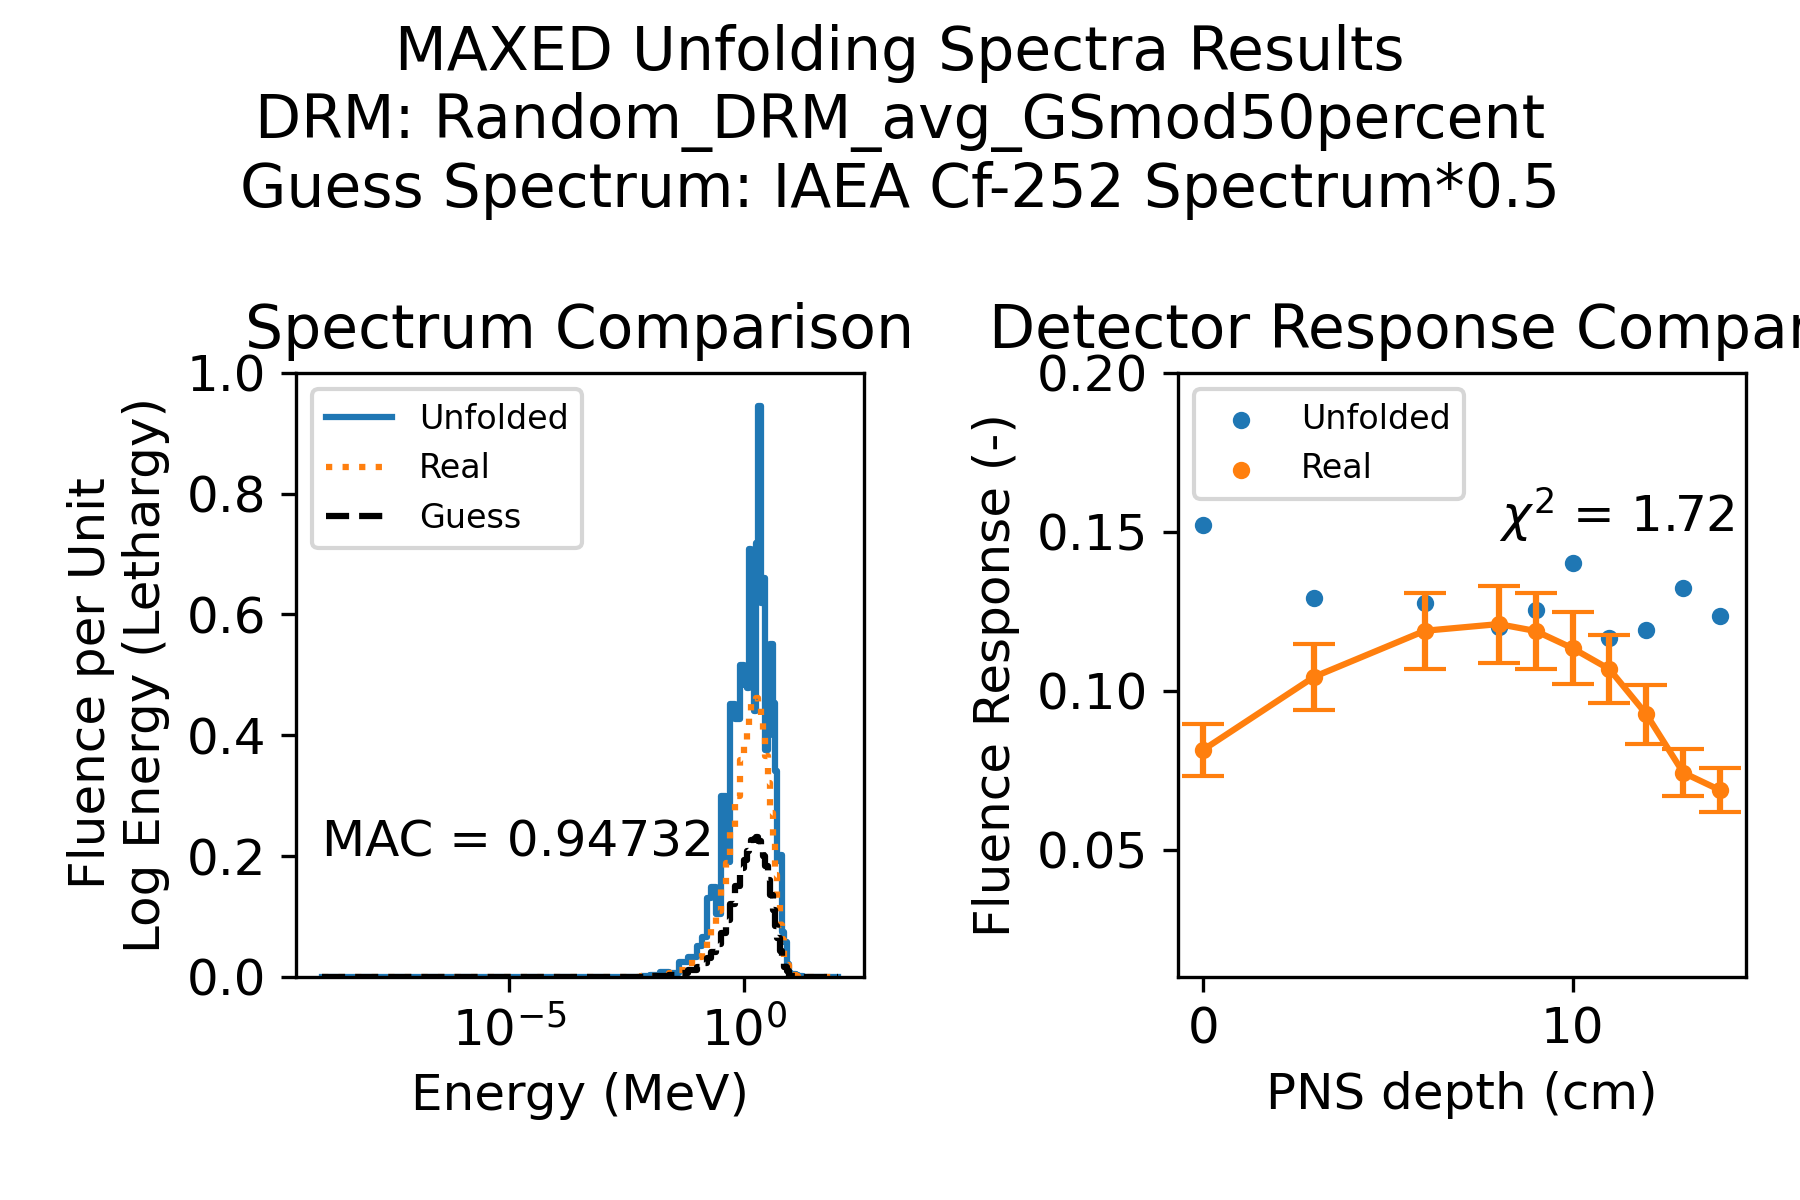
\includegraphics[scale=0.8]{images/Random_DRM_avg_GSmod50percent_IAEA Cf-252 Spectrum_0.png}
  \caption{The results of the MAXED algorithm using a modified Cf-252 guess spectrum and a randomly generated DRM.} \label{MAXED_result_randomDRM_gs50Cf}
\end{figure}

\subsection*{Thoughts on MAXED}
When given very good information, the MAXED algorithm can perform neutron spectrum unfolding. This is highly dependent on the operator who provides the information to the algorithm. As shown in the examples above, the results of MAXED do not depart greatly from the initial guess spectrum. 

At first, it appears that a randomly generated DRM performs well, but I think this is an artifact of the limitations of the MAXED algorithm. I believe that there are a great many local minima and the initial guess makes a very big impact. Additionally, when the guess spectrum is modified like in earlier examples, the effects of the randomness are more pronounced.   % Chapter 2

\newpage
%\input{Chapter3} % Chapter 3

%   .
%   .
%   .

\newpage
\chapter{Conclusions}\label{chap_conc}

This is your final chapter. 
It does not have to be titled ``Conclusions"; it could be ``Discussion", or whatever else you prefer.

I am going to use this chapter to talk about references.
All your references should be in the references.bib file, in the same folder as this source file.
Only entries that are actually referenced in the text will show up, so you do not have to delete entries from the references.bib file.
References will appear in the order they are cited in the text.
You can look at the references.bib file to see how to enter each of the references in the following examples.

For papers in proceedings you need: authors' names, title of paper, title of proceedings, location [city, state (if in the US), or city, country (if abroad)], dates (month, days, year).
See examples in \cite{proc1,proc2,proc3}.

For papers in journals you need: authors' names, title of paper, full name of journal, volume, number (if exists), pages, year.
See examples in \cite{artic1,artic2,artic3}.

For book chapters or papers in books you need: authors' names, title of chapter or paper, title of book, name of editors, name of publisher, pages, year.
See examples in \cite{chapter1,chapter2,chapter3}.

For books you need: authors' names, title of book, name of publisher, year.
See examples in \cite{book1,book2,book3}.  % Conclusion Stuff

%************************************************
%************************************************

    %
    % If you have appendices in your dissertation, you will need the
    % following, else keep it commented. The following appendices should be in
    % files called ``app1.tex'' and ``app2.tex'', and they
    % look just like any chapter. You may rename it as you want.
    %

\appendix
\chapter{This is an Appendix}\label{app1}

You can have as many appendices as needed.
%\include{app2}

%************************************************
%************************************************


%
% The all important bibliography file at the end of your document!! 
% I have already set the preferred style; do not change it unless necessary.
% Examples of how to use them are given in the ``conclusion" chapter
% of this document.

\printbibliography

\end{document}


